\let\negmedspace\undefined
\let\negthickspace\undefined
\documentclass[journal]{IEEEtran}
\usepackage[a5paper, margin=10mm, onecolumn]{geometry}
%\usepackage{lmodern} % Ensure lmodern is loaded for pdflatex
\usepackage{tfrupee} % Include tfrupee package

\setlength{\headheight}{1cm} % Set the height of the header box
\setlength{\headsep}{0mm}  % Set the distance between the header box and the top of the text

\usepackage{gvv-book}
\usepackage{gvv}
\usepackage{cite}
\usepackage{amsmath,amssymb,amsfonts,amsthm}
\usepackage{algorithmic}
\usepackage{graphicx}
\usepackage{textcomp}
\usepackage{xcolor}
\usepackage{txfonts}
\usepackage{listings}
\usepackage{enumitem}
\usepackage{mathtools}
\usepackage{gensymb}
\usepackage{comment}
\usepackage[breaklinks=true]{hyperref}
\usepackage{tkz-euclide} 
\usepackage{listings}
% \usepackage{gvv}                                        
\def\inputGnumericTable{}                                 
\usepackage[latin1]{inputenc}                                
\usepackage{color}                                            
\usepackage{array}                                            
\usepackage{longtable}                                       
\usepackage{calc}                                             
\usepackage{multirow}                                         
\usepackage{hhline}                                           
\usepackage{ifthen}                                           
\usepackage{lscape}
\begin{document}

\bibliographystyle{IEEEtran}
\vspace{3cm}

\title{12.8.ex.13}
\author{EE24BTECH11014 - Deepak Ahirwar}

% \maketitle
% \newpage
% \bigskip
{\let\newpage\relax\maketitle}

\renewcommand{\thefigure}{\theenumi}
\renewcommand{\thetable}{\theenumi}
\setlength{\intextsep}{10pt} % Space between text and floats

\textbf{Question:}\\

Find the area bounded by the curve $y =\cos{x}$ between $x = 0$ and $x = 2 \pi$.

\solution:\\


\textbf{Theoretical logic:}
\begin{enumerate}
    \item \textbf{Set up the integral:} \\
    The area under the curve can be calculated as:
    \begin{align}
        \text{Area} = \int_{x_1}^{x_2} f(x) \, dx
    \end{align}
    Here:
    \begin{align}
        f(x) = \cos(x), \quad x_1 = 0, \quad x_2 = 2\pi
    \end{align}
    Check whether the curve \( y = \cos(x) \) crosses the x-axis in the interval \( x \in [0, 2\pi] \):
    \begin{align}
        y = 0 = \cos(x) \implies x = \frac{\pi}{2}, \frac{3\pi}{2}
    \end{align}
    Thus, the integral becomes:
    \begin{align}
        \text{Area} &= \int_0^{\pi/2} \cos(x) \, dx 
        - \int_{\pi/2}^{3\pi/2} \cos(x) \, dx 
        + \int_{3\pi/2}^{2\pi} \cos(x) \, dx
    \end{align}
    
    \item \textbf{Compute each integral:}
    \begin{align}
        \int_0^{\pi/2} \cos(x) \, dx &= \left[\sin(x)\right]_0^{\pi/2} = \sin\left(\frac{\pi}{2}\right) - \sin(0) = 1 - 0 = 1 \\
        \int_{\pi/2}^{3\pi/2} \cos(x) \, dx &= \left[\sin(x)\right]_{\pi/2}^{3\pi/2} = \sin\left(\frac{3\pi}{2}\right) - \sin\left(\frac{\pi}{2}\right) = -1 - 1 = -2 \\
        \int_{3\pi/2}^{2\pi} \cos(x) \, dx &= \left[\sin(x)\right]_{3\pi/2}^{2\pi} = \sin(2\pi) - \sin\left(\frac{3\pi}{2}\right) = 0 - (-1) = 1
    \end{align}

    \item \textbf{Add the areas:}
    \begin{align}
        \text{Area} &= 1 + |{-2}| + 1 \\
        &= 1 + 2 + 1 = 4
    \end{align}
\end{enumerate}

The total area bounded by the curve \( y = \cos(x) \) between \( x = 0 \) and \( x = 2\pi \) is $4$

\textbf{Computational Logic:} 
Using the trapezoidal rule to get the area. The trapezoidal rule is as follows.
\begin{align}
    \int^{b}_{a} f\brak{x}dx\approx \sum^{N}_{k=1}\frac{f\brak{x_{k+1}}+f\brak{x_{k}}}{2}h
\end{align}
where
\begin{align}
    h=\frac{b-a}{N}
\end{align}
$\therefore$The difference equation obtained is\\
\begin{align}
    A &= \int_a^b f\brak{x}\, dx \approx h\brak{\frac{1}{2}f\brak{a} + f\brak{x_1} + f\brak{x_2} \cdots + f\brak{x_{n-1}} + \frac{1}{2}f\brak{b}}\\
    h &= \frac{b-a}{n}\\
    A &= j_n, \text{ where, } j_{i + 1} = j_i + h\frac{f\brak{x_{i+1}} + f\brak{x_i}}{2}\\ 
        \xrightarrow{} j_{i + 1} &= j_i + h\brak{{x_{+1}^2}+{x_{i}^2}}\\
    x_{i+1} &= x_i + h\\
    n&=100000
\end{align}
Using the code answer obtained is 4.0000000000
\begin{figure}[h]
    \centering
    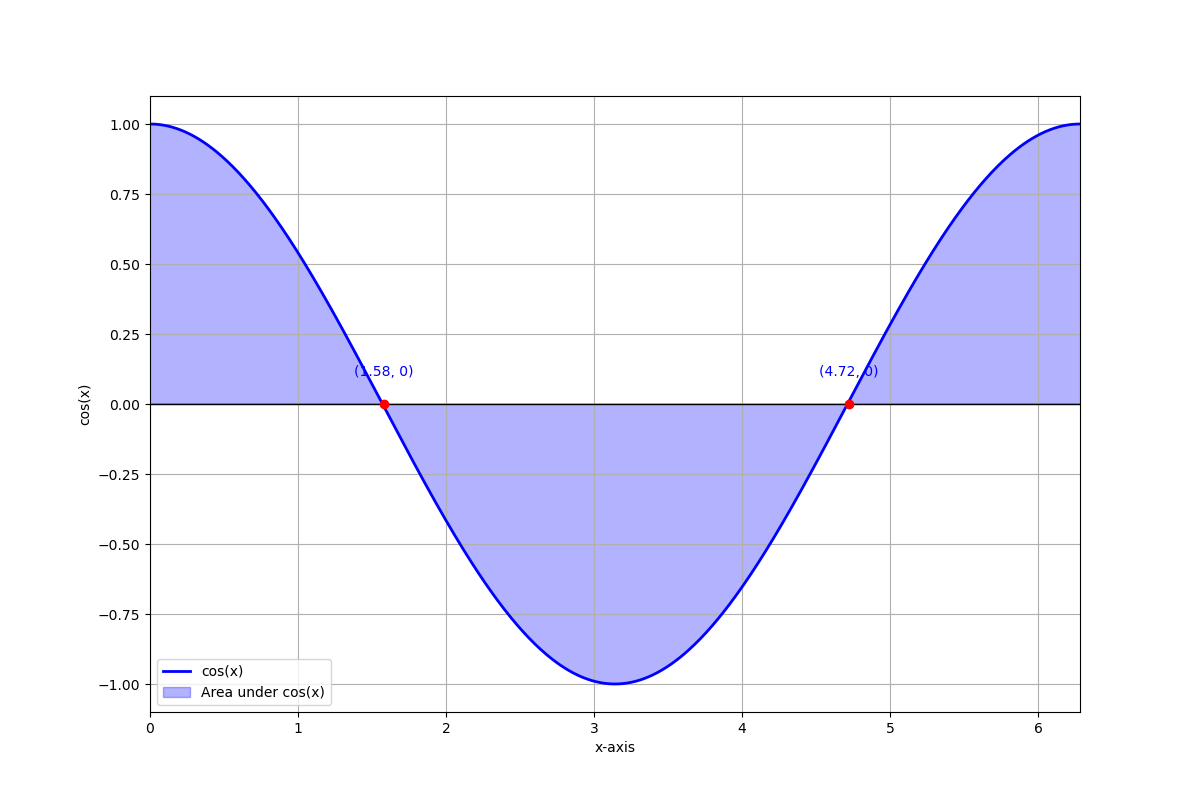
\includegraphics[width=\columnwidth]{fig/figs.png}
 \end{figure}




\end{document}
